\section{非理想反应器的计算}


\begin{frame}
    \frametitle{轴向扩散模型的计算}

    以一级反应为例，对关键组分A做物料衡算，输入 - 输出 - 消耗 = 0
    \[
        D_{\mathrm{a}} \frac{\mathrm{d}^{2} c_{\mathrm{A}}}{\mathrm{d} Z^{2}}-u \frac{\mathrm{d} c_{\mathrm{A}}}{\mathrm{d} Z}-k c_{\mathrm{A}}=0
    \]
    
    \[
       \text{结合边界条件} \qquad \qquad \qquad  Z=0, u c_{\mathrm{A} 0}=u c_{\mathrm{A}}-\left.D_{\mathrm{a}} \frac{\mathrm{d} c_{\mathrm{A}}}{\mathrm{d} Z}\right|_{0^{+}} \qquad \qquad \qquad \qquad \quad
    \]
    \[
        Z=L_{\mathrm{r}},\left.\frac{\mathrm{d} c_{\mathrm{A}}}{\mathrm{d} Z}\right|_{L_{\mathrm{r}}^{-}}=0
    \]
    解析求解得
    \[
        \frac{c_{\mathrm{A}}}{c_{\mathrm{A} 0}}=\frac{4 \alpha}{(1+\alpha)^{2} \exp \left[-\frac{P e}{2}(1-\alpha)\right]-(1-\alpha)^{2} \exp \left[-\frac{P e}{2}(1+\alpha)\right]}
    \]
    \[
        \text{式中} \qquad \alpha=(1+4 k \tau / P e)^{1 / 2}
    \]

\end{frame}


\begin{frame}
    \frametitle{轴向扩散模型的计算}

    当$Pe \to \infty$时，$\alpha \to 1$，因此可将$\alpha$展开成
    \[
        \alpha=1+\frac{1}{2}\left(\frac{4 k \tau}{P e}\right)-\frac{1}{8}\left(\frac{4 k \tau}{P e}\right)^{2}+\cdots
    \]
    代回，得
    \[
        c_{\mathrm{A}} / c_{\mathrm{A} 0}=\exp (-k \tau)
    \]
    当$Pe \to 0$时，
    \[
        \frac{c_{\mathrm{A}}}{c_{\mathrm{A} 0}}=\frac{4 \alpha}{(1+\alpha)^{2}\left(1-\frac{P e}{2}+\alpha \frac{P e}{2}\right)-(1-\alpha)^{2}\left(1-\frac{P e}{2}-\alpha \frac{P e}{2}\right)}
    \]
    \[
        =\frac{4 \alpha}{4 \alpha-\alpha P e+\alpha^{3} P e}=\frac{1}{1+k \tau} \qquad \qquad \qquad \qquad
    \]
    这与连续釜式反应器进行一级反应时的计算式一样。

\end{frame}


\begin{frame}
    \frametitle{轴向扩散模型，一级反应}
    \begin{minipage}{0.38\linewidth}
        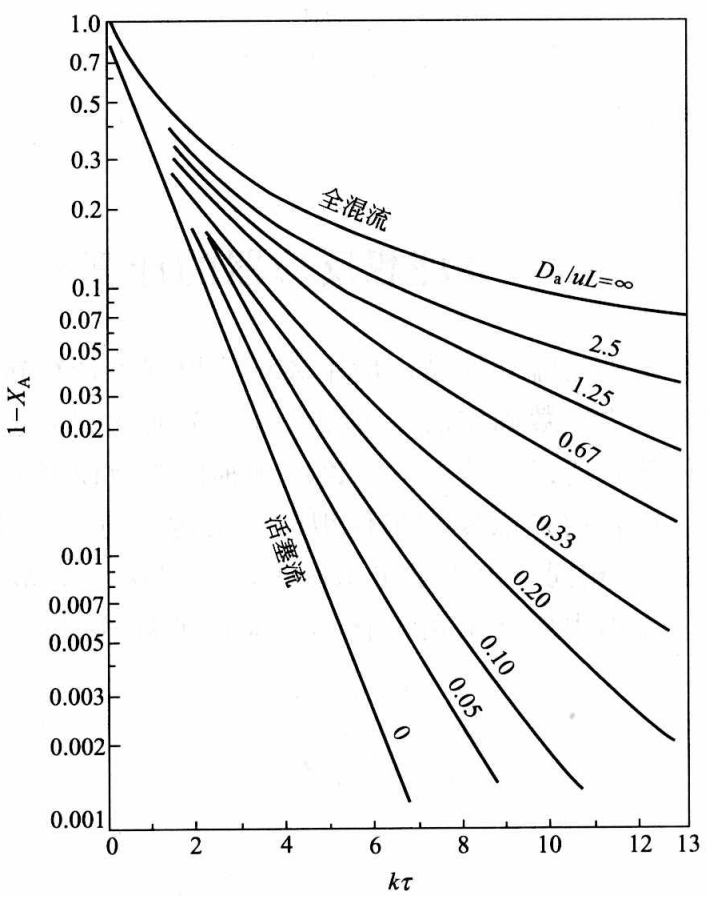
\includegraphics[width=\linewidth]{figures/fig5.23.png}
    \end{minipage}\hfill
    \begin{minipage}{0.6\linewidth}
        \begin{itemize}
            \item 具有闭式边界条件的轴向扩散模型，根据模型参数$Pe$的取值不同，可以体现从活塞流到全混流之间的任何返混情况。
            \item 实际反应器的转化率随$Pe$倒数的减小而增加。
            \item 空时越大，流动状况偏离理想流动的影响也越大。
        \end{itemize}
    \end{minipage}   

\end{frame}


\begin{frame}
    \frametitle{轴向扩散模型，二级反应}
    \begin{minipage}{0.72\linewidth}
        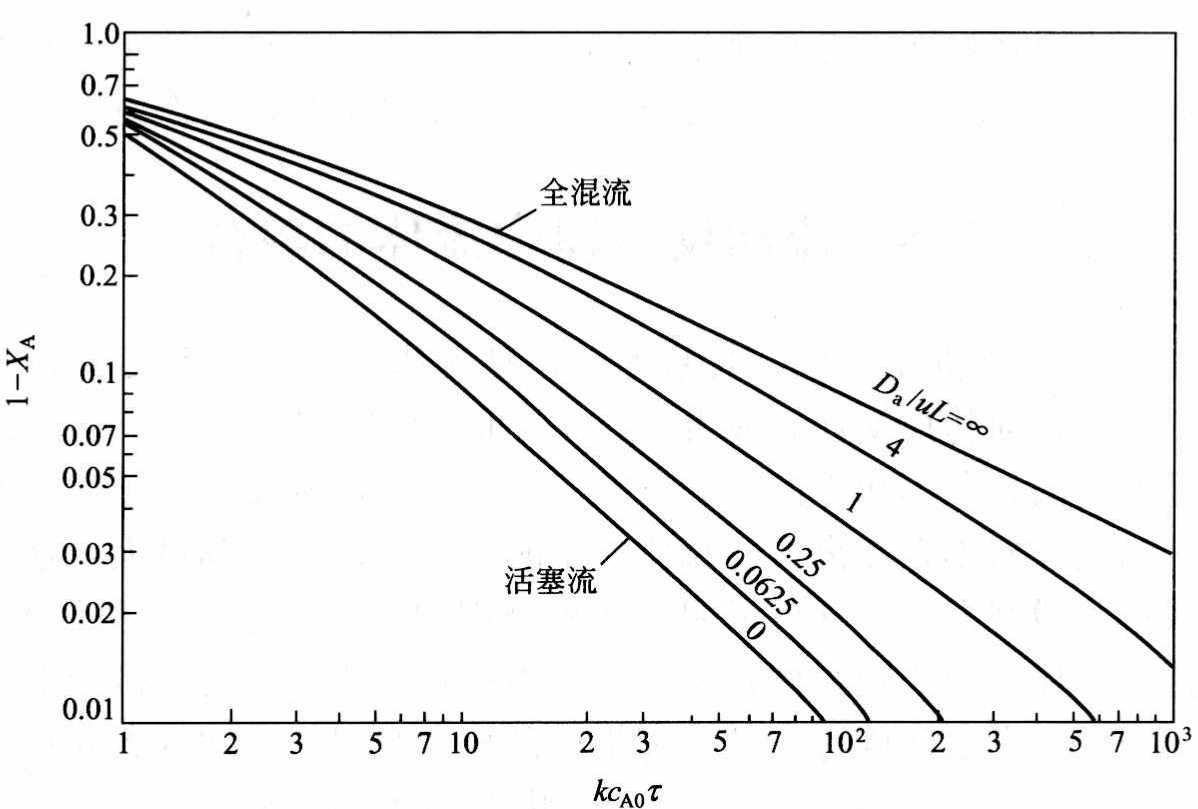
\includegraphics[width=\linewidth]{figures/fig5.24.png}
    \end{minipage}
    \begin{minipage}{0.264\linewidth}
        \begin{itemize}
            \item 在其他条件相同的情况下，二级反应的转化率受返混的影响比一级反应大。
            \item 一般而言，反应级数越高，返混对反应结果的影响越大。
        \end{itemize}
    \end{minipage}   

\end{frame}
